\documentclass[border=3pt,tikz]{standalone}
\usepackage{amsmath}
\usetikzlibrary{calc}
\usetikzlibrary{arrows.meta} % for arrow size
\begin{document}

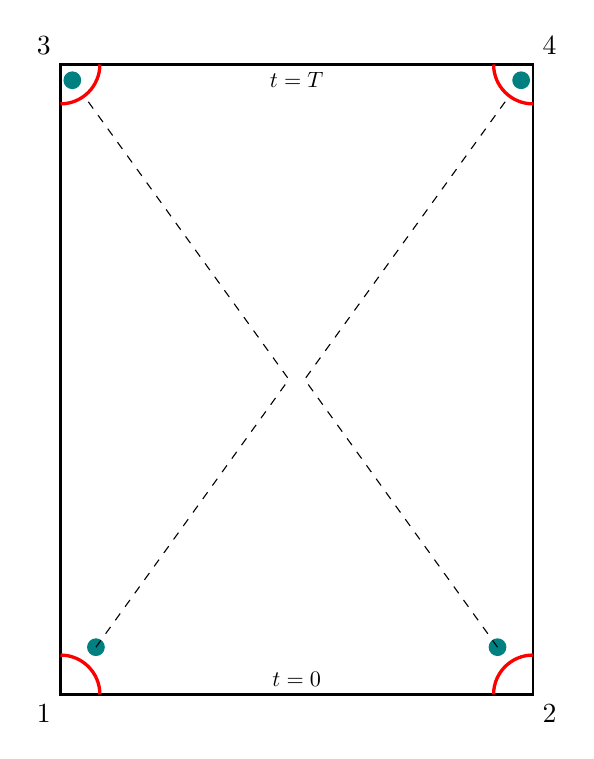
\begin{tikzpicture}[scale=1.0]
    \usetikzlibrary {arrows.meta}
    \usetikzlibrary {calc}
    
    \draw[thick] (0, 0)  -- (6, 0) -- (6, 8) -- (0, 8) -- cycle;
    \node [below left] at (0, 0) {$1$};
    \node [below right] at (6, 0) {$2$};
    \node [above left] at (0, 8) {$3$};
    \node [above right] at (6, 8) {$4$};
    
    \draw[very thick, red] (0.5, 0) arc (0:90:0.5);
    \draw[very thick,red] (5.5, 0) arc (180:90:0.5);
    \draw[very thick,red] (6, 7.5) arc (270:180:0.5);
    \draw[very thick,red] (0, 7.5) arc (270:360:0.5);
    
    \filldraw[teal] (0.45, 0.6) circle (3pt) ;
    \draw[dashed] (0.45, 0.6) -- (2.9, 4) -- (0.3, 7.6);
    \filldraw[teal] (0.15, 7.8) circle (3pt) ;
    
    
    \filldraw[teal] (5.55, 0.6) circle (3pt) ;
    \draw[dashed] (5.55, 0.6) -- (3.1, 4) -- (5.7, 7.6);
    \filldraw[teal] (5.85, 7.8) circle (3pt) ;
    
    \node[above, scale=0.8] at (3, 0) {$t=0$};
    \node[below, scale=0.8] at (3, 8) {$t=T$};
    
    \end{tikzpicture}
    \end{document}